\section{Performanzanalyse}
Die Performanz der Entropiefunktion hängt von vielen Faktoren ab. Wir wenden trotzdem einige Optimierungen an, die in der Theorie die Performanz verbessern sollen. In dieser Abschnitt geht es darum, wie unsere Optimierungen auf die Performanz auswirkt.

Die erste Optimierung liegt an SIMD Prinzip. Die Entropiefunktion lässt sich sehr einfach vektorisieren, außer der Verwendung von log2f-glibc und der Lookup-Tabelle.

Um unnötige Überprüfungen in unsere SIMD-Implmentation zu vermeiden, erweitern wir das Array der Fließkommazahlen, sodass die Länge durch 4 trennbar ist. Die zusätzliche Zahlen sind alle $0$ und sie verändern nicht das Endergebnis. Außerdem allozieren wir das Array 16-Byte-Aligned, dann können wir Befehle, wie z.B. \emph{movaps}, nutzen, die effizienter sind als ihre unaligned Gegenstücke.

% can be removed
Wir speichern die Konstanten für die Remez und Artanh Approximations im Speicher in der Reihenfolge der Verwendung. Das führt zu schnelleren Speciherzugriffen, weil dann die Konstanten in Cache geladen und von der Cache gelesen werden können.

% Eine andere Optimierung ist Software-Pipelining in Logarithmusfunktionen. Wir versuchen die Pipeline so zu unterstützen, dass die unabhängigen arithmetischen Operationen einander nicht blockieren. Assembly Implementation lässt der Pipelining besser helfen.

In allen Implementationen behandeln wir die Spezialfälle nicht, nämlich NaN, $\pm$Inf, $\pm$0 und negative Zahlen nicht. Der Grund ist wir stellen uns in der Entropiefunktion sicher, dass in die Log-Funktion eingegebener Wert immer im Interval $[0,1]$ liegt. Wenn der Wert $0$ ist, spielt das Ergebnis von der Log-Funkiton keine Rolle denn es wird später mit $0$ multipliziert. Damit sparen wir einige Branches in der Funktion, was gut auf die Performanz wirkt.

Unsere Logartihmusfunktionen sind stark für Entropieberechnung spezialisiert. Dazu lassen wir in der Assembly Implementation einige ABI Konventionen aus. Wir sichern Caller-Saved Registern in Entropiefunktion nicht denn wir wissen genau welche Registern in der Log-Funktion geändert wird. Dies erlaubt einen bemerkenswerten Gewinn an der Performanz.

\begin{figure}[h]
    \centering
    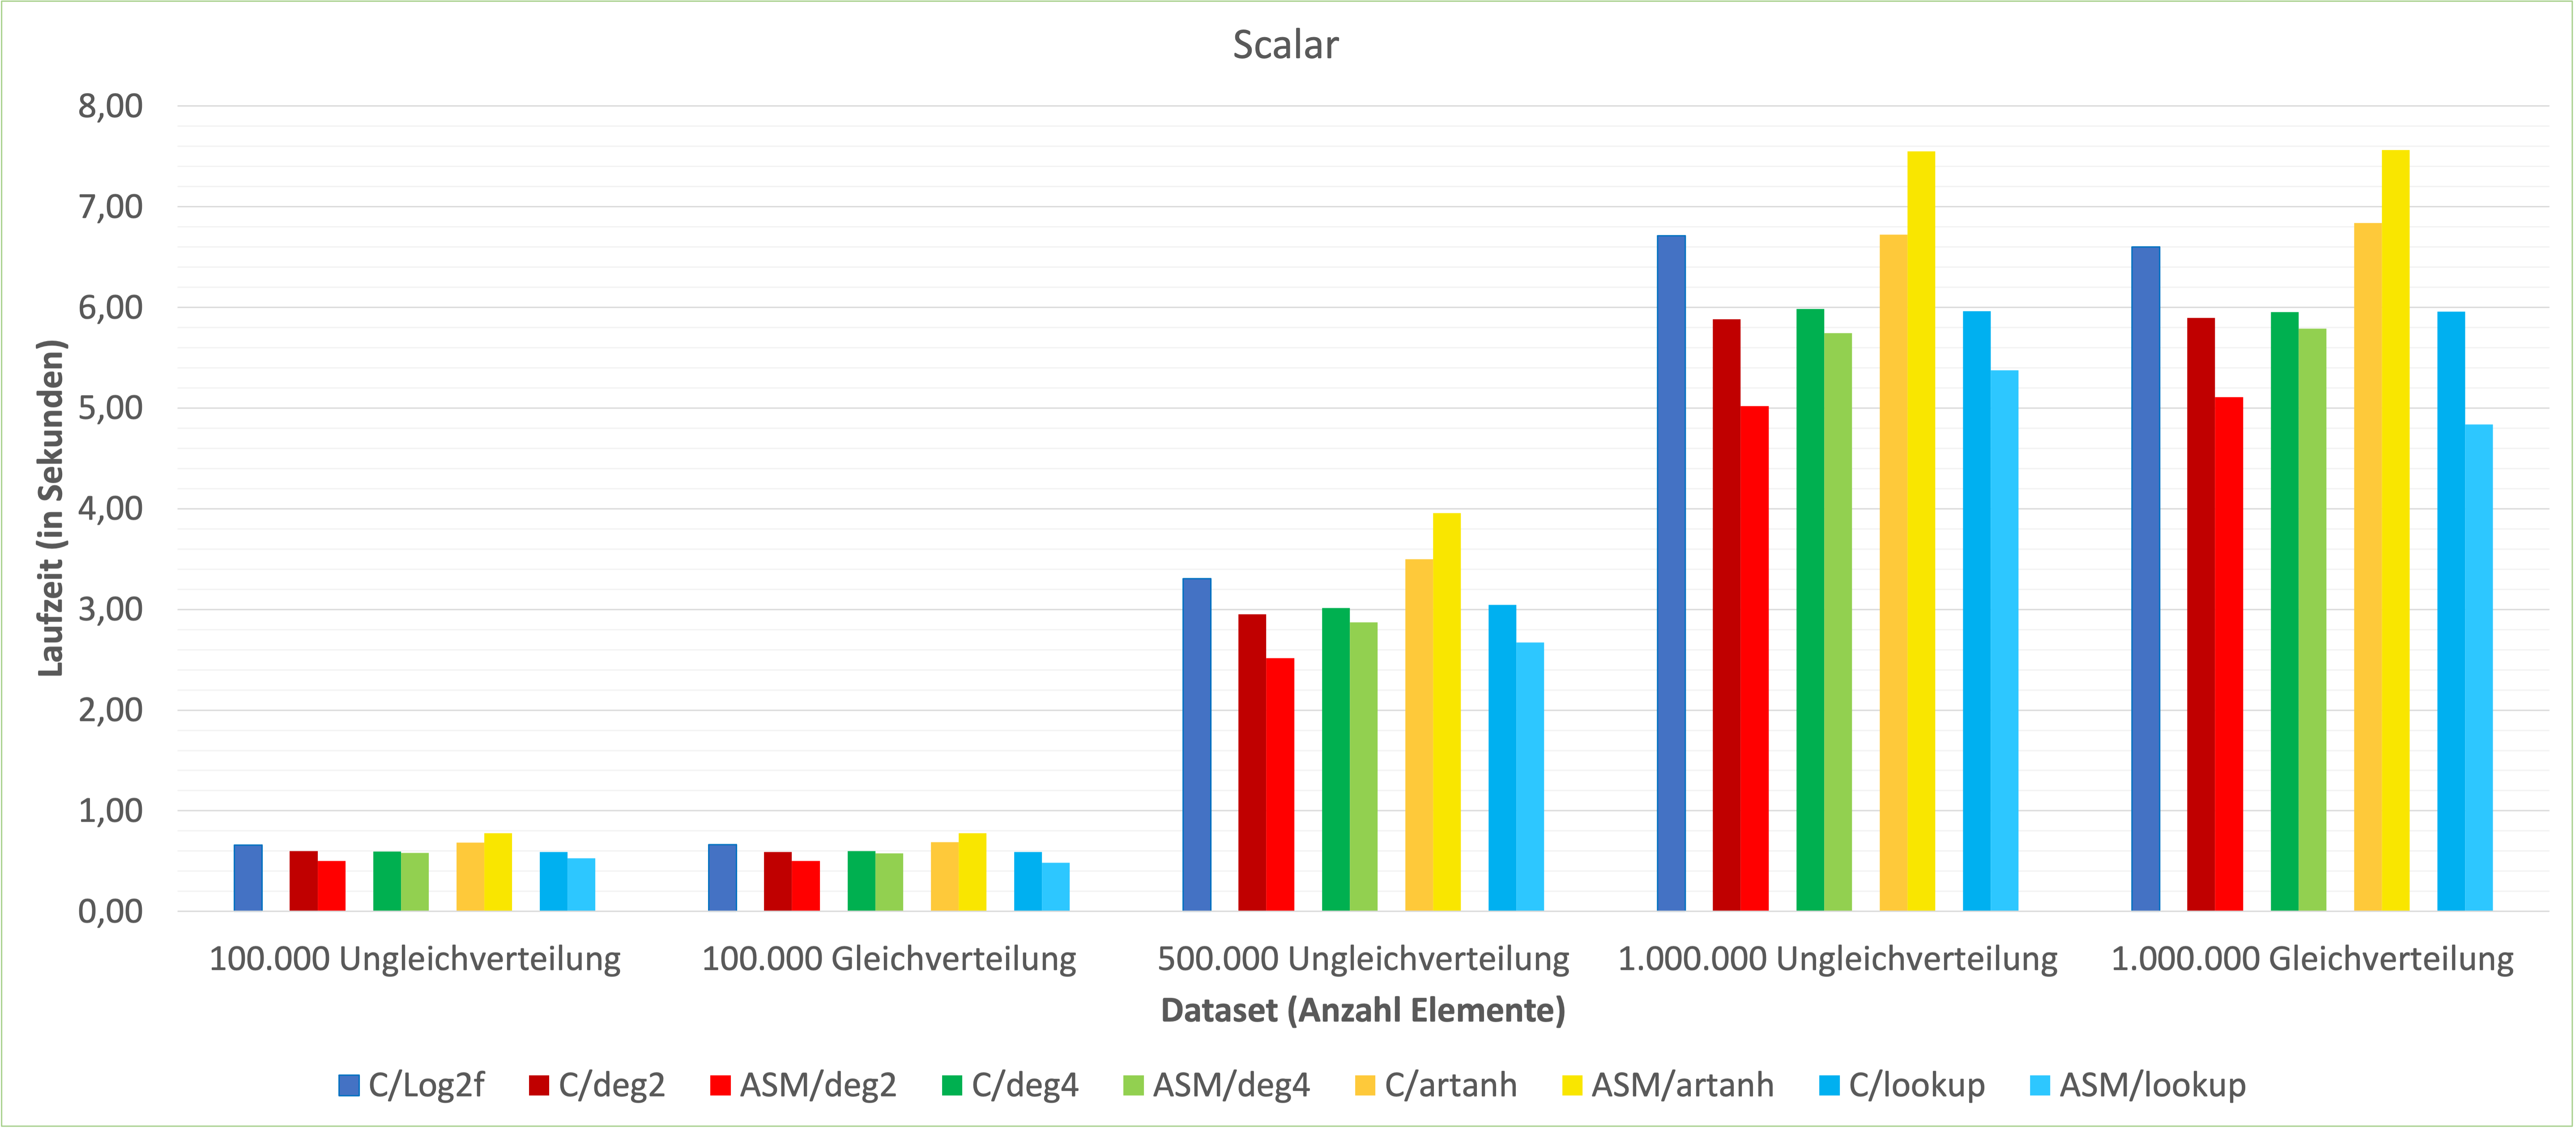
\includegraphics[scale=0.3]{graph_scalar.png}
    \caption{Performazgrafik zu skalarer Implementation mit 1000 Iterationen}
    \label{fig:graph_scalar}
\end{figure}

\begin{figure}[h]
    \centering
    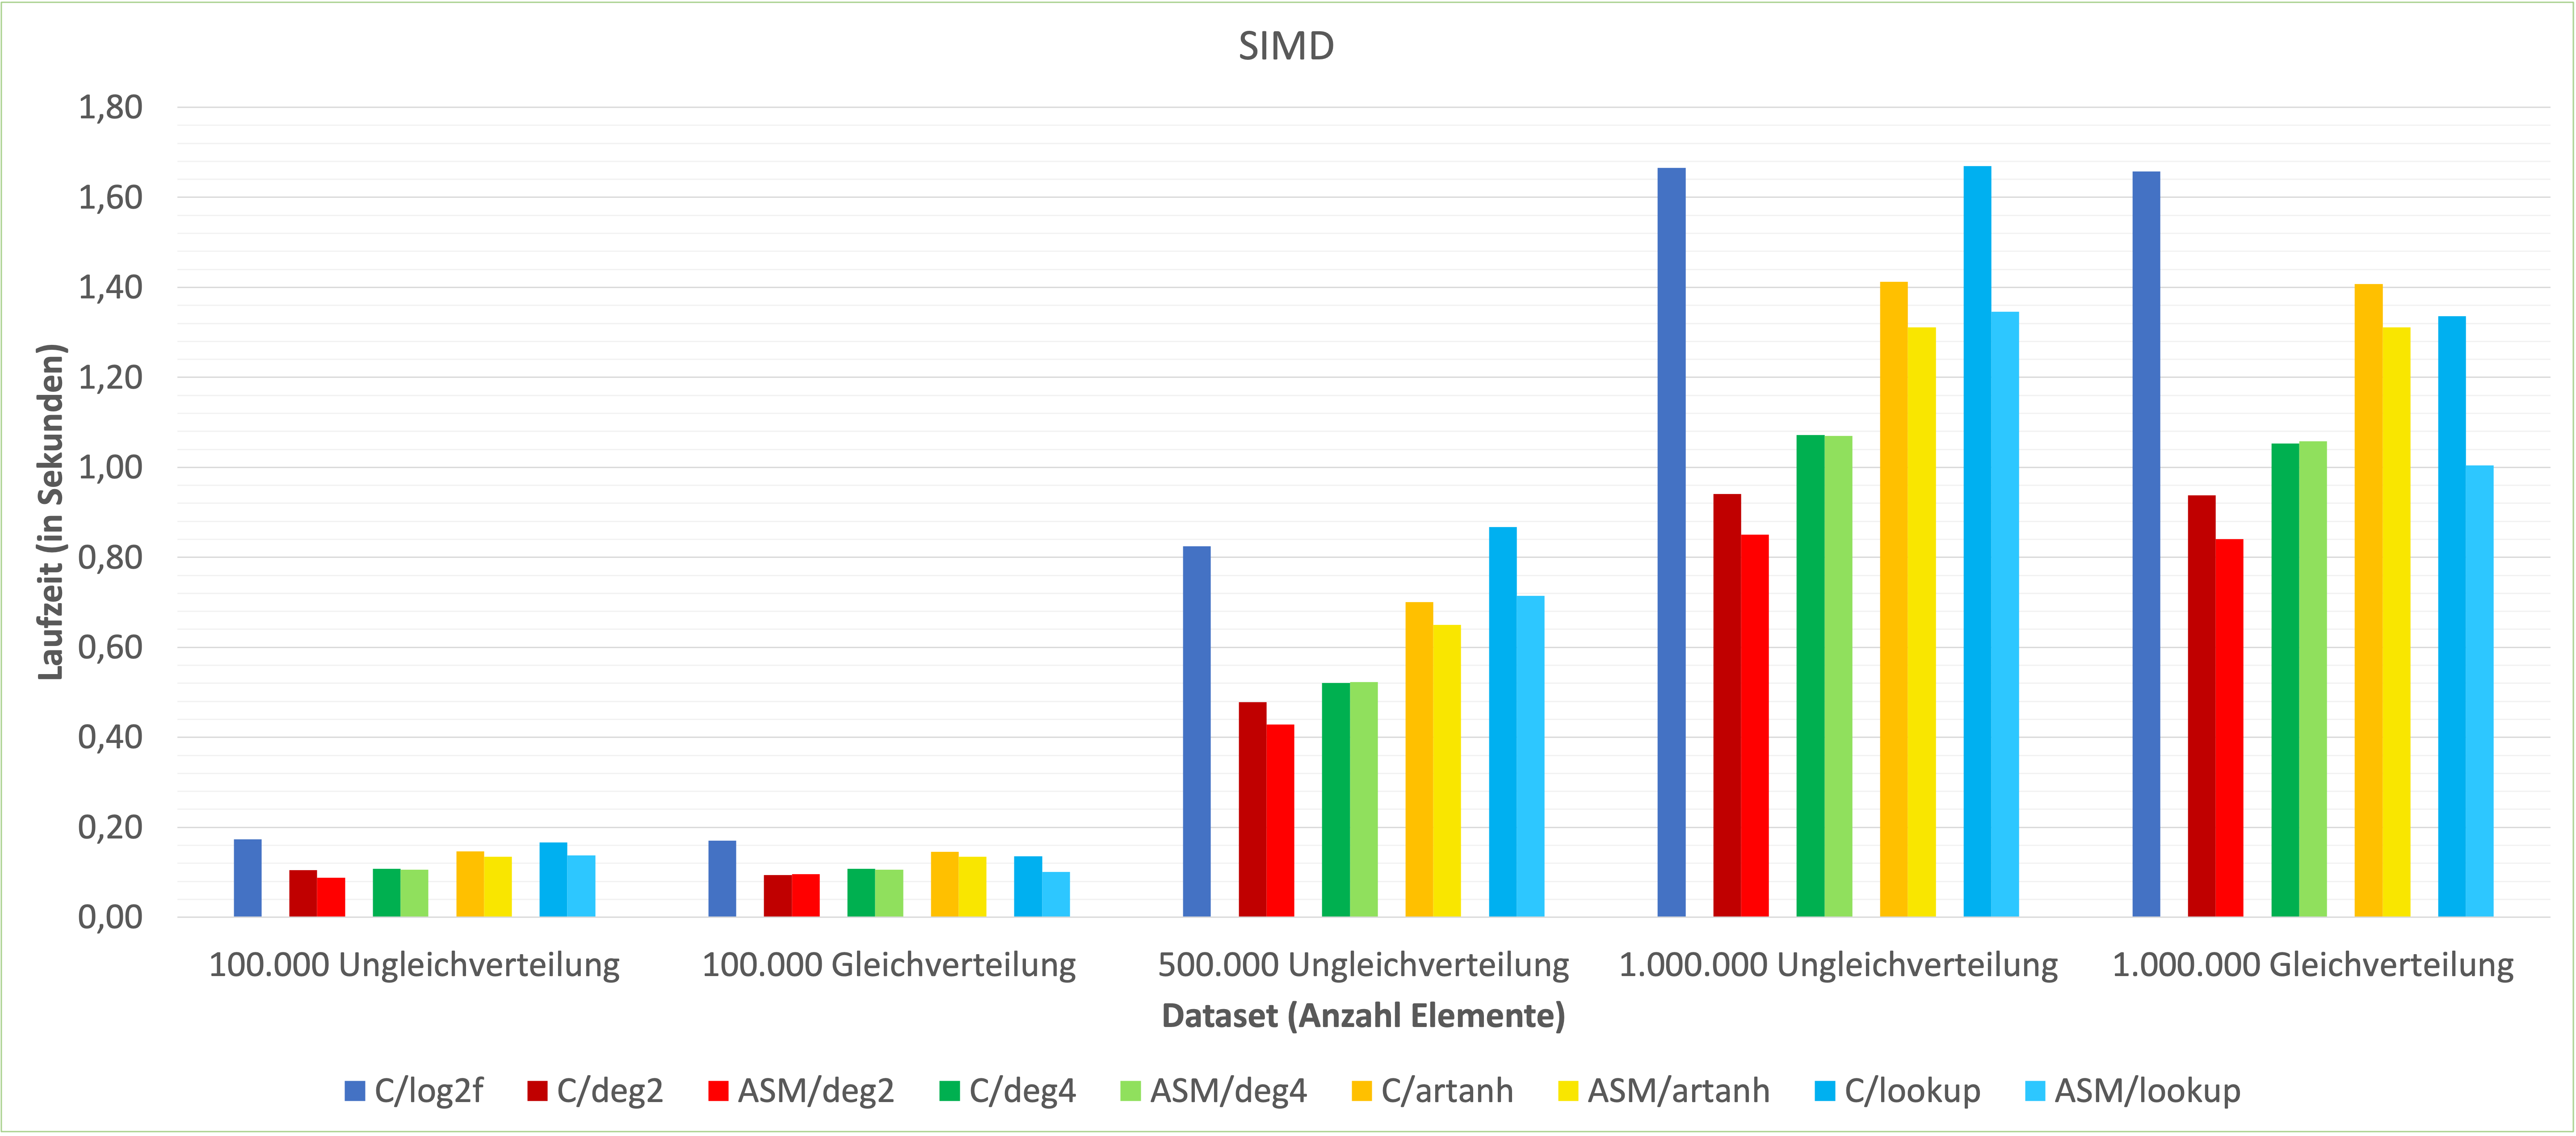
\includegraphics[scale=0.3]{graph_simd.png}
    \caption{Performazgrafik zu SIMD Implementation mit 1000 Iterationen}
    \label{fig:graph_simd}
\end{figure}

Um Grafiken zu erstellen, haben wir das Programm mit GCC 11.2 und Flag $-O3$ kompiliert und die Zeitmessungen auf Arch Linux 3.2 mit Kernel Version 5.12.8 - Intel i7-10750H @ 2.6 GHz mit $1000$ Iterationen durchgeführt.

In den Grafiken ist es zu sehen, dass unsere Logarithmusfunktionen leistungsfähiger als glibc Implementation. Darüber hinaus sind wir in der Lage, mittels Assembly unsere Funktionen noch besser als C implementieren.

Die Logarithmusfunktion mit Lookup Tabelle ist etwas schneller mit Gleichverteilungen gegen Ungleichverteilungen. Dies liegt daran, dass bei der Gleichverteilung immer der gleiche Wert von der Cache abgefragt wird.

\begin{figure}[h]
    \centering
    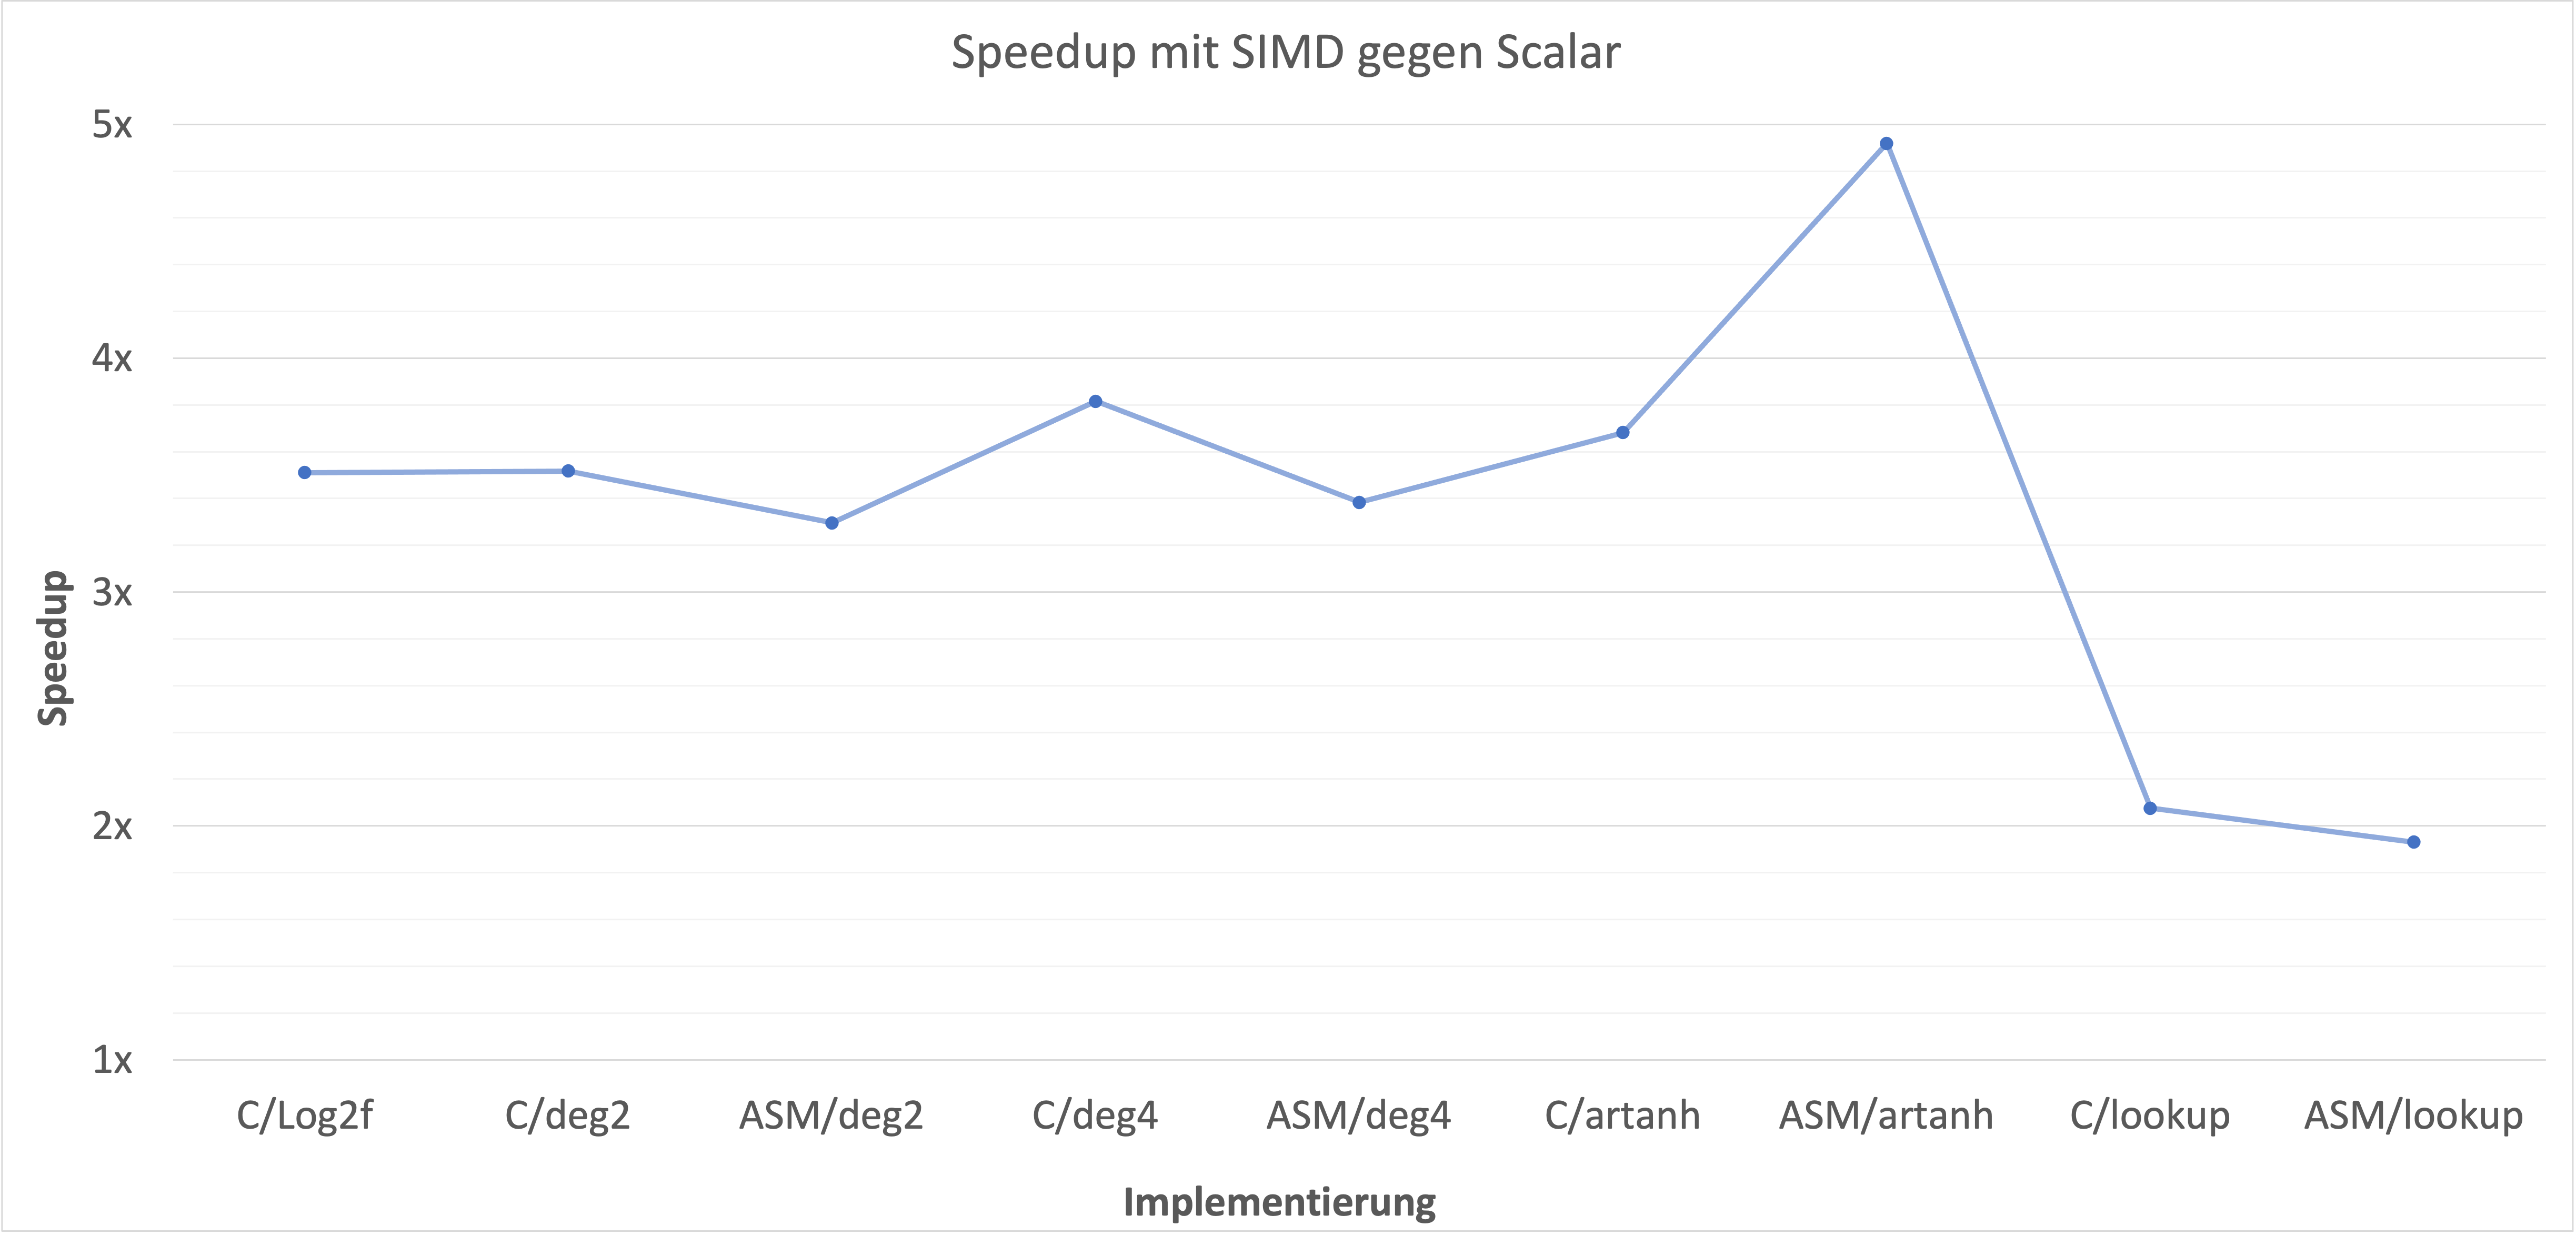
\includegraphics[scale=0.35]{graph_speedup.png}
    \caption{Speedup mit SIMD Implementation}
    \label{fig:graph_speedup}
\end{figure}

Obwohl die Glibc-Implementierung der Logarithmusfunktion ebenfalls eine Lookup-Tabelle verwendet, erreichen wir einen Speedup von $3.5$. Der Grund dafür ist, dass, da die Lookup Tabelle eine Größe von 16 hat, fast alle Werte immer im Cache sind. Ein weiterer Grund ist, dass wir nicht auf Sonderfälle  NaN, $\pm$Inf, $\pm$0 und negative Zahlen überprüfen, was uns einige Branches erspart.

Das durchschnittliche Speedup, das wir mittels unserer SIMD-Implementiereung außer Lookup-Tabelle ist $3.5$. Zusätzlich ist die Speedup bei der Lookup Tabelle mittels SIMD gegen Skalar fast 2 Mal wegen der notwendigen Speicherzugriffe.